The field-effect transistor (FET) has become a promising transducer for sensors and biosensors in recent years. Its superior electronic properties, which come from its ability to amplify the signal, make it very appealing for the detection of molecules with high sensitivity \citep{xuFlexible2022, yuRecent2024}. Before getting to the FET that is in use today, it had to undergo significant developments; the main milestones are herein described, to underline the improvements in fabrication techniques and materials, which have resulted in enhanced performance, reduced size, and that led to a wide range of electronic applications \citep{ahmadEvolution2021,tanAdvancements2024}.

\paragraph{A Brief History of the field-effect transistor}
Many electronics applications nowadays rely on the FET, including analog and digital circuits \citep{kimIntegrated2011, fortunatoOxide2012, yanRecent2022}, amplifiers, mixers and modulators \citep{torricelliIntegrated2021, yanRecent2022, pasadasExploiting2023}, and finally (bio)sensors \citep{shkodraElectrolytegated2021, dengSensors2022}.


Since their development in the 1950s, field-effect transistors have been extensively used in electronics, from analog and digital circuits \citep{kimIntegrated2011, fortunatoOxide2012, yanRecent2022} to radio frequency applications like amplifiers, mixers, and modulators \citep{torricelliIntegrated2021, yanRecent2022, pasadasExploiting2023}, and even sensing and biosensing \citep{shkodraElectrolytegated2021, dengSensors2022}.

The first transistors, referred to as \vv{semiconductor triodes}, were structurally resembling vacuum tube triodes, having three terminals in common, namely emitter, base, and collector \citep{bardeenTransistor1948}. The innovation was replacing the vacuum tube with a semiconductor to allow electron flow. Shortly after, field-effect transistors (FETs) were developed, based on the ideas of Edgar Julius Lilienfeld \citep{edgarDevice1933, edgarMethod1930}, with the electrodes now called gate, source, and drain. By applying a voltage to the gate, an electric field was able to control the charge density and conductivity in the semiconductor channel \citep{shockleyUnipolar1952}.

Kahng and Atalla at Bell Laboratories introduced the Metal-Oxide-Semiconductor FET (MOSFET) in 1960, by adding a silicon dioxide layer between the silicon semiconductor and the gate. This insulating layer is what made integrated circuits possible thanks to a lower power consumption, a higher input impedance, and device miniaturization \citep{kahngSiliconSilicon1960,atallaNew1962,kilbyMiniaturized1964}.

Soon after, thin-film transistors (TFTs) emerged as a significant variant of FETs. TFTs were first fabricated by Paul Weimer by means of thin film deposition, namely evaporation \citep{weimerTFT1962}: differently from MOSFETs, Weimer used an insulating glass substrate, onto which he patterned Au electrodes and deposited a layer of cadmium sulfide as semiconductor, insulated from the gate by silicon monoxide. TFTs, compared to MOSFETs, often use alternative semiconductors, including amorphous metal oxides or organic compounds \citep{pettiMetal2016}. Despite their typically lower carrier mobility compared to MOSFETs, TFTs are widely utilized in applications such as display systems, power transmission, and data transmission, with their flexibility expanding their range of possible applications \citep{pettiMetal2016}.

In 1968, Complementary Metal-Oxide-Semiconductor (CMOS) technology was introduced, combining n-channel and p-channel MOSFETs to create energy-efficient circuits \citep{wanlassNanowatt1963}. All together these advancements led to the development of Moore's law in \num{1965}, which states that transistor density and computing power should double every two years \citep{mooreCramming1965}.

Another transistor revolution began in more recent times. As transistors began to approach physical limits approximately ten years ago, their scaling slowed, deviating from Moore's predictions \citep{Intel}; this lead to the study of wide-bandgap semiconductors like gallium nitride (GaN) \citep{arakawaProgress2002, lidowEnhancement2011} and silicon carbide (SiC) aiming for higher power densities and efficiency \citep{bhatnagarComparison1993, chenMOS2010}. These new materials address issues like heat dissipation and short-channel effects and make it possible to employ FETs in advanced systems, such as quantum computers \citep{chhowallaTwodimensional2016, chenPerformance2024, niuSuperconducting2024}.

\paragraph{Field-effect transistor: components and materials}

\begin{figure}[ht]
	\centering
	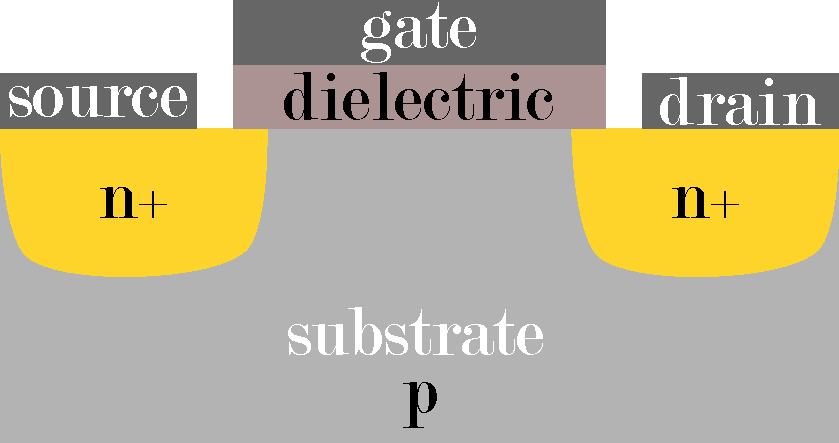
\includegraphics[width=0.3\textwidth]{figures/chapter1/fet/Fig3_FETstructure.pdf}
	\caption{Schematic representation of a field-effect transistor (FET). The device consists of a p-type substrate (body) onto which n+ source and drain electrodes are fabricated. A dielectric layer separates the gate from the semiconducting channel. The gate has the role of controller by modulating the amount of charge carriers that accumulate at the semiconductor-dielectric interface, thus enabling the formation of a channel between source and drain.}
	\label{fig:FETstructure}
\end{figure}

The previous paragraph introduced the source, drain, and gate as the three eletrotrodes of FETs, which are built on a semiconductor material, as seen in Figure \ref{fig:FETstructure}. Between the source and drain is the semiconducting channel, where charge carriers flow, namely electrons (for n-type semiconductors) and holes (for p-type semiconductors), whose concentration is controlled by the gate and the field effect that results from an applied voltage \citep{liChemical2019, shkodraElectrolytegated2021}. However, other phenomena also produce changes in the output current, \eg{} variations in surface effects, local electric fields, and chemical reactions near the device surface \citep{sangProgress2016, shkodraElectrolytegated2021}.

A crucial aspect of FET fabrication is the selection of materials for each component, as these determine the electrical performance and device stability.
The first choice to make for fabricating FETs is the substrate, which can be chosen among a wide range of materials, including silicon, flexible polymers (\eg{} PET, polyimide), cellulose-based materials, and more.
The next layer is made by the electrodes, which are fabricated with conductive materials, most often metals such as gold (Au), silver (Ag), titanium (Ti), chromium (Cr), and more.
The dielectric material must then be chosen, as it has a central role in the functioning of FETs, separating the gate from the semiconductor channel. This insulating layer, \eg{} silicon dioxide in MOSFETs, prevents direct current flow between the gate and the channel, while still allowing modulation of channel conductivity through electric field-induced polarization \citep{ortizHighk2010, wangHighk2018}.
The last element, \ie{} the semiconductor, must be selected wisely, as it greatly influences the current in tne channel.
To date, the most widely used semiconductor is silicon, particularly in MOSFETs, owing to its excellent electrical properties and manufacturability, including its scalability and processability \citep{zahoorCarbon2023, heywangSilicon2004, guptaSemiconductor2016}. Nonetheless, ongoing efforts aim to move toward new, increasingly efficient materials with higher carrier mobility and improved electrostatic properties at small dimensions, such as III-V semiconductors, which possess wide bandgap and are able to enhance device performance \citep{chelliahCurrent2017, delalamoNanometrescale2011}. More commonly widespread are organic, inorganic and carbon-based alternatives, which are herein briefly described. Organic semiconductors, which include polythiophenes and blends, are generally cost-effective, flexible and possess good electrical properties that make them attractive to use in organic light-emitting diodes (OLEDs), flexible electronics, and organic photovoltaics \citep{facchettiSemiconductors2007, jacobsControlling2017, rootMechanical2017}.
As for carbon-based materials, the most widely employed in transistors are graphene \citep{krsihnaRecent2021, moonGraphene2012, reddyGraphene2011} and carbon nanotubes (CNTs) \citep{kumarCarbon2023, maqboolReview2024, shkodraElectrolytegated2021}. In particular, graphene is a carbon allotrope in which the atoms are arranged in a hexagonal structure with \ce{sp^2} hybridization. This geometry and the single-atom thickness confer to graphene properties such as a large surface area, high carrier mobility, and excellent thermal conductivity, in conjunction to a high resistance to mechanical stresses, while maintaining flexibility \citep{farjadianRecent2020, radsarGraphene2021, uradeGraphene2023}.

\paragraph{A focus on carbon nanotubes}
\begin{figure}[h]
    \centering
    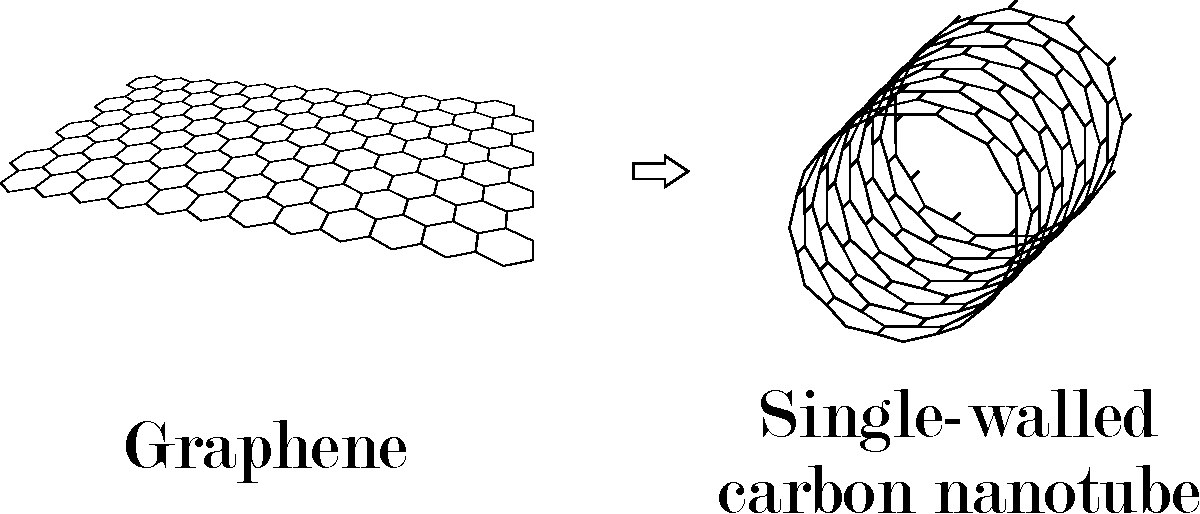
\includegraphics[width=0.5\textwidth]{figures/chapter1/fet/Fig4_cntStructure.pdf}
    \caption{Drawing of a single-walled carbon nanotube (SWCNT), which derives from the wrapping of a graphene sheet into a cylinder form.}
    \label{fig:cntStructure}
\end{figure}

In the search for alternative semiconductors to silicon, carbon nanotubes are repeatedely found in literature. These are one-dimensional structures derived from a graphene sheet rolled into a cylinder \citep{iijimaHelical1991}, as seen in Figure~\ref{fig:cntStructure}. Depending on the wrapping angle, CNTs can have three different geometries, namely armchair, zig-zag, and chiral, which exhibit distinct physical and electrical properties, \eg{} they can have either metallic or semiconducting behavior \citep{dresselhausChapter1996, avourisMolecular2002, popovCarbon2004}. CNTs can also be classified based on the number of concentric cylinders they possess, which also impacts their properties and allows for a wide range of applications \citep{popovCarbon2004}. These materials derive their unique electrical characteristics from both the graphene sheet and their cylindrical shape; indeed they retain the thermal conductivity and strength from graphene, while the wrapping causes electron confinement which leads to quantization of electron momentum \citep{avourisMolecular2002, mceuenSinglewalled2002}. This effect is particularly noticeable in semiconducting single-walled carbon nanotubes (SWCNTs), which exhibit very high mobilities and transconductances, making SWCNTs more desirable than traditional semiconductors \citep{mceuenElectron2004}. 
